\input{preamble}
\usepackage{eurosym}
\usetikzlibrary {datavisualization}

\begin{document}

\pagestyle{fancy}
\fancyhead[L]{Terminale STMG}
\fancyhead[C]{\textbf{TD n°5-2 : statistiques à deux variables}}
\fancyhead[R]{\today}

%Inventé

\exe{}{
Une entreprise étudie ses coûts unitaires de production (variable $y$) en fonction du nombre d'article produit (variable $x$) :
 \begin{center}
  \begin{tabular}{|l|*{10}{c|}}
	 \hline
	 \textbf{Production : $x_i$} & 50 & 55 & 60 & 65 & 70 & 75 & 80 & 85 & 90 & 100 \\
	 \hline
	 \textbf{Coûts : $y_i$} & 58 & 71 & 94 & 110 & 122 & 139 & 147 & 167 & 188 & 221 \\
	 \hline
	\end{tabular}
 \end{center}
 
On a représenté dans le repère ci-dessous le nuage de points associé à cette série statistique :
  
\begin{tikzpicture}
\begin{axis}%
    [
        grid=major,  
        x=2mm,
        y=0.5mm,
        xtick={50,55,...,100},   
        xmin=50,
        xmax=110,
        xlabel={\small $x$},
        axis x line=middle,
        ytick={50,60,...,230},
        tick label style={font=\small},
        ymin=50,
        ymax=230,
        ylabel={\small $y$},
        axis y line=middle,
        no markers,
        samples=100,
    ]
\addplot[teal, only marks] 
table[x=x,y=y, col sep=comma] {data_TD5_3.csv};
\end{axis}
\end{tikzpicture}

\begin{enumerate}
  \item Calculer les coordonnées du point moyen G de ce nuage de points. Placer G sur le graphique.
  \item \begin{enumerate}
	 \item Justifier qu'il est pertinent de réaliser un ajustement affine pour ce nuage de points.
	 \item Déterminer une équation de la droite $\Delta$ d'ajustement affine de $y$ en $x$ obtenue par la méthode des moindres
	 carrés, sous la forme $y=ax+b$.
	 On arrondira les paramètres à $10^{-1}$ près.
	\end{enumerate}
	\item Vérifier que la droite $\Delta$ passe par G.
	\item À l'aide de cet ajustement affine, estimer la valeur de $y$ pour $x = 150$.
	\item Déterminer la production permettant de minimiser les coûts estimés. \\
	\textit{Indication : le coût total est de $x \times y$, exprimer $y$ en fonction de $x$ et étudier la fonction obtenue.}
 \end{enumerate}
 
}{exe:1}{
\begin{enumerate}
  \item $G(73 ; 131,7)$
  \item \begin{enumerate}
	 \item Les données présentent une tendance linéaire.
	 \item $a \approx 3,20$ et $b \approx -102$.
	\end{enumerate}
	\item Par définition, $b = \bar{y} - a \bar{x}$ donc, pour $x = \bar{x}$, l'ordonnée correspondante est 
	\begin{align*}
	y & = a \bar{x} + b \\
	& = a \bar{x} + \bar{y} - a \bar{x} \\
	& = \bar{y} .
	\end{align*}
	Donc la droite $(\Delta)$ passe par $G(\bar{x}, \bar{y})$.
	\item Pour $x = 150, y \approx 3,20 \times 150 - 102 \approx 378$.
	\item Déterminer la production permettant de minimiser les coûts estimés.
	\textit On étudie la fonction $c(x) = x \times y \approx 3,20 x^2 - 102 x$. \\
	 Sa dérivée est $c'(x) \approx 6,40 x -102$ qui s'annule en $x \approx \dfrac{102}{6,40}$. \\
	 On dresse le tableau de variation :
	 \begin{center}
		\begin{tikzpicture}
		   \tkzTabInit{$x$ / 1 , $c'(x)$ / 1, $c(x)$ / 1.5}{$0$, $102/6.40$, $\infty$}
		   \tkzTabLine{, -, z, +,}
		   \tkzTabVar{+/ , -/, +/ }
		\end{tikzpicture}
	\end{center}	
	Le coût unitaire minimal est donc atteint pour une production $\dfrac{102}{6,40} \approx 16$ unités. \\
	Cependant le coût correspondant $c(16) \approx 3,20 \times 16^2 - 102 \times 16$ est négatif ce qui n'a pas de sens ! \\
	Conclusion : un modèle statistique n'est pas le réel, il peut présenter des limites.
\end{enumerate}
}

\newpage

% Manuel
\exe{}{
Une entreprise fabrique un équipement. Le prix de revient théorique de fabrication (variable $y$) se répartit en $a$ euros de frais fixes
et $b$ euros par unité produite.

\begin{enumerate}

\item Exprimer, en fonction du nombre $n$ d’unités produites, le prix de revient théorique d’une unité. \\
\textit{Le coût de revient correspond au coût total par unité produite. Il faut donc tenir compte des frais fixes et unitaires.} \\
Dans la suite de l’exercice, on propose une méthode de recherche des coefficients $a$ et $b$.

\item Dans la pratique, on a relevé les chiffres portés dans le tableau ci-dessous et on a représenté le nuage de points 
$M_i(n_i, y_i)$ dans un repère. Un ajustement affine paraît-il justifié ?

 \begin{center}
  \begin{tabular}{|l|*{10}{c|}}
	 \hline
	 \textbf{$n_i$} & 1 & 2 & 3 & 4 & 5 & 6 & 7 & 8 & 9 & 10 \\
	 \hline
	 \textbf{$y_i$} & 1504 & 809 & 540 & 438 & 375 & 320 & 290 & 254 & 231 & 212 \\
	 \hline
	\end{tabular}
 \end{center}
 

\begin{center}
\begin{tikzpicture}
\begin{axis}
    [
        grid=major,  
        x=10mm,
        y=0.04mm,
        xtick={0,1,...,10},   
        xmin=0,
        xmax=10,
        xlabel={\small $n$},
        axis x line=middle,
        ytick={0,200,...,1600},
        tick label style={font=\small},
        ymin=0,
        ymax=1600,
        ylabel={\small $y$},
        axis y line=middle,
        no markers,
        samples=100,
    ]
\addplot[teal, only marks] 
table[x=x,y=y, col sep=comma] {data_TD5_4.csv};
\end{axis}
\end{tikzpicture}
\end{center}

\item Pour $i$ allant de 1 à 10, on pose $x_i = \dfrac{1}{n_i}$.



\begin{enumerate}
\item Calculer les valeurs approchées des valeurs $x_i$ à $10^{-2}$ près et les présenter dans un tableau avec les valeurs de $y_i$, sur le modèle de la question précédente.

\item Représenter le nuage de points $P_i$ de coordonnées $(x_i \, ; \, y_i)$ dans un repère orthogonal, en prenant pour unités graphiques :
\begin{itemize}
    \item en abscisses : 1 cm pour 0,1 unité ;
    \item en ordonnées : 1 cm pour 100 \euro.
\end{itemize}

\item Un ajustement affine paraît-il justifié ?
\end{enumerate}

\item 

\begin{enumerate}
\item Déterminer une équation de la droite $\Delta$ d'ajustement affine de $y$ en $x$ obtenue par la méthode des moindres carrés,
sous la forme $y=ax+b$. On arrondira les paramètres à $10^{-2}$ près. Tracer cette droite dans le repère.

\item En déduire les valeurs approchées des nombres $a$ et $b$ de la question 1.

\item Quelle estimation peut-on donner du prix de revient d’une unité de l’équipement si on en fabrique 20 ?
\end{enumerate}

\end{enumerate}
}{exe:2}{
\begin{enumerate}

\item Le prix de revient théorique d'une unité correspond au prix de revient pour $n$ unités, divisé par le nombre d'unités soit :
\[ p = \dfrac{a + b \cdot n}{n} = a \cdot \dfrac{1}{n} + b . \]

\item Non, les points ne présentent pas de tendance linéaire.

\item 

\begin{enumerate}
\item


 \begin{center}
  \begin{tabular}{|l|*{10}{c|}}
	 \hline
	 \textbf{$x_i$} & 1 & 0,5 & 0,33 & 0,25 & 0,2 & 0,17 & 0,14 & 0,13 & 0,11 & 0,1 \\
	 \hline
	 \textbf{$y_i$} & 1504 & 809 & 540 & 438 & 375 & 320 & 290 & 254 & 231 & 212 \\
	 \hline
	\end{tabular}
 \end{center}

\item 

\begin{center}
\begin{tikzpicture}
\begin{axis}
    [
        grid=major,  
        x=100mm,
        y=0.04mm,
        xtick={0,0.1,...,1},   
        xmin=0,
        xmax=1.1,
        xlabel={\small $x$},
        axis x line=middle,
        ytick={0,200,...,1600},
        tick label style={font=\small},
        ymin=0,
        ymax=1600,
        ylabel={\small $y$},
        axis y line=middle,
        no markers,
        samples=100,
    ]
\addplot[teal, only marks] 
table[x=x,y=y, col sep=comma] {data_TD5_4_correc.csv};
\end{axis}
\end{tikzpicture}
\end{center}

\item Oui, les points présentent bien une tendance linéaire
\end{enumerate}

\item 

\begin{enumerate}
\item $a \approx 1432,11$ et $b \approx 77,69$.
\item Comme $y \approx ax+b$ avec $x=\dfrac{1}{n}$ on a $a \approx 1432,11$ et $b \approx 77,69$ 
(ce sont ceux calculés précédemment)

\item Environ 149,30 \euro.
\end{enumerate}

\end{enumerate}
}

%%%%%%%%%%%%%%%%%%%%%%%%%%%%%

\newpage
\fancyhead[C]{\textbf{Solutions - TD5-2}}
\shipoutAnswer

\end{document}